\chapter{Trabalho Proposto}

    Neste capítulo será abordado a metodologia utilizada neste trabalho, bem como os objetivos e o cronograma.

    \section{Metodologia}
        Motivado pelo propósito de experienciar o processo científico, este trabalho seguiu a seguinte metodologia: 
        
        \begin{enumerate}[label=\alph*)]
            \item Identificação do Problema: a partir da análise do trabalho de Jurak~\cite{JURAK2020} foi possível observar que evasão de colisão aplicado a USV é uma demanda atual, e que a identificação de situações de colisão é uma necessidade em tais sistemas. Com isso, originou-se a pergunta de pesquisa que guiará este trabalho:
            
            \vspace{3mm}
            
            \centerline{\textit{"Como identificar situações de colisões no âmbito de USVs?"}}
            
            \item Definição da Sentença de Busca: a partir da pergunta formulada na etapa anterior, obteve-se o entendimento de quais áreas seriam permeadas para responde-la. Com esse entendimento, extraiu-se as palavras chaves formulando a seguinte sentença de busca:
            
            \vspace{3mm}
            
            \centerline{\textit{"USV" AND "COLREGS" AND "collision avoidance"}}
            
            \item Seleção de Trabalhos Relacionados: aplicando a sentença de busca definida em bases de busca como IEEE Explorer\footnote{https://ieeexplore.ieee.org/Xplore/home.jsp}, Scopus\footnote{https://www.scopus.com/search/form.uri?display=basic} e Science Direct\footnote{https://www.sciencedirect.com/}, foi realizada a pré-seleção de trabalhos que poderiam embasar o trabalho proposto. A pré-seleção foi feita com base na leitura do \textit{"abstract"} do trabalho e da dissertação acerca de evasão de colisão e CPA, resultando em 28 trabalhos pré-selecionados. Posteriormente, através de uma análise mais detalhada dos trabalhos, para identificar as técnicas utilizadas, e de seus respectivos Índice H, foram selecionados os 5 trabalhos mais relevantes para serem utilizados como referência neste trabalho.
            
            \item Leitura dos Trabalhos Selecionados e Extração de Conhecimentos Relevantes: para obter um conhecimento mais aprofundado a respeito da área, do problema e das técnicas utilizadas pelos autores atualmente, foi realizada uma primeira leitura dos trabalhos atentando para a fundamentação teórica e analisando brevemente seus resultados. Com isso foi possível compreender como implementar CPA e quais resultados esperar da implementação.
            
            \item Estruturar a Proposta de Trabalho: com o conhecimento obtido da etapa anterior foi possível estruturar a presente proposta de trabalho contendo uma contextualização, embasamento teórico, objetivos e os meios que serão utilizados para atingi-los.
            
            \item Implementação da Proposta Aceita: com a proposta analisada e aprovada pelos avaliadores, será realizada a implementação do CPA e a integração com o sistema desenvolvido por Jurak~\cite{JURAK2020}, seguindo o cronograma apresentado na Figura~\ref{fig:chap3_schedule}.
            
            \item Executar Casos de Testes: validar a implementação realizada a partir de casos específicos de testes, a fim de estressar a implementação e obter possíveis comportamentos não previstos durante a implementação do sistema.
            
            \item Analise dos Resultados: analisar o comportamento obtido na fase de testes e compará-lo com o comportamento anterior à implementação deste trabalho. Também será realizada uma comparação com os resultados obtidos pelos demais autores da área. 
        \end{enumerate}
        
    \section{Objetivos}
        O principal objetivo deste trabalho é desenvolver um componente de software capaz de identificar situações de colisão entre embarcações através do método CPA, dado a posição e a velocidade das embarcações envolvidas. Além disso, será realizada a implementação do VO a fim de criar obstáculos virtuais seguindo o mesmo padrão apresentado por Jurak~\cite{JURAK2020} em seu sistema. Como contribuição, essa aplicação será integrada ao sistema desenvolvido por Jurak~\cite{JURAK2020} a fim de aprimorá-lo bem como para testar a implementação realizada neste trabalho. Com isso, será possível que um encontro com uma configuração (posições) prevista pela COLREGS não tenha a regra aplicada devido à velocidade das embarcações. Entretanto, não é desejável que o sistema omita a aplicação de uma COLREGS em uma situação de colisão. 
        
        Como objetivo secundário, para evitar a omissão da aplicação de uma COLREGS em uma situação de risco, serão realizados testes unitários para validar que o comportamento obtido está de acordo com o esperado. Também serão realizadas análises com o objetivo de verificar o impacto ocasionado pela implementação deste trabalho no esforço computacional requerido pelo sistema. Como objetivo final, realizar-se-a um comparativo entre os resultados obtidos com o novo comportamento do sistema e os resultados anteriores à implementação deste trabalho. Além disso, comparações com resultados obtidos pelos autores da literatura de referência também serão realizadas.
        
    \section{Cronograma}
        A Figura~\ref{fig:chap3_schedule} apresenta detalhadamente o cronograma de atividades, previstas e já realizadas, para atingir os objetivos expostos nesse documento. O planejamento foi realizado considerando atividades por semana e prevê, de forma geral, as seguintes atividades:
        \begin{enumerate}
            \item \textbf{Entregas (Escrita)}:
            \item \textbf{Estudo da Literatura}:
            \item \textbf{Estudo do Framework de Desenvolvimento}:
            \item \textbf{Implementação}:
            \item \textbf{Coleta e Análise dos Resultados}:
        \end{enumerate}
        
        \begin{figure}[htb]
            \centering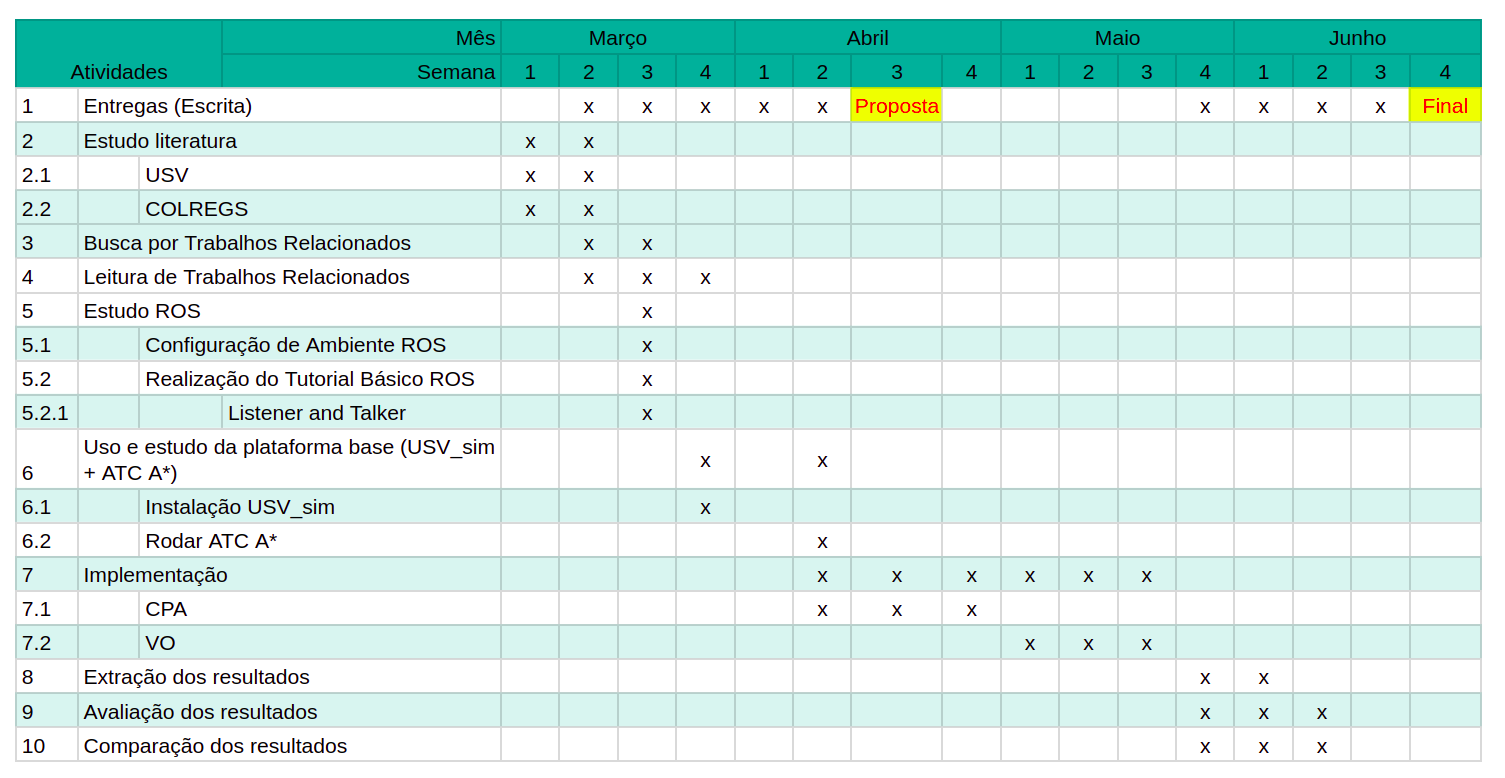
\includegraphics[width=1.3\textwidth, angle=90]{fig/chap3/schedule.png}
            \caption{\label{fig:chap3_schedule} Cronograma proposto para realização das atividades.}
        \end{figure}